% Full system architecture: DenPAR -> derived labels -> the train/inference fork -> severity -> evaluation.
% The claim this figure exists to make: the keypoint heads are TRAINED on ground-truth boxes
% but EVALUATED on YOLO boxes, and that fork is a named contributor to the ICC gap.
\documentclass[border=6pt,multi,tikz]{standalone}
\usepackage{amsmath}
\usepackage{helvet}
\renewcommand{\familydefault}{\sfdefault}
\usetikzlibrary{positioning,arrows.meta,calc,fit,backgrounds,shapes.geometric,
                decorations.pathreplacing,decorations.pathmorphing,patterns}

\definecolor{ink}{HTML}{1D2433}
\definecolor{muted}{HTML}{6B7280}
\definecolor{accent}{HTML}{D62828}
\definecolor{good}{HTML}{2A9D8F}
\definecolor{soft}{HTML}{E8ECF1}
\definecolor{edge}{HTML}{AAB3C0}
\definecolor{lane}{HTML}{F4F6F9}
\definecolor{trainc}{HTML}{3A6EA5}

\begin{document}
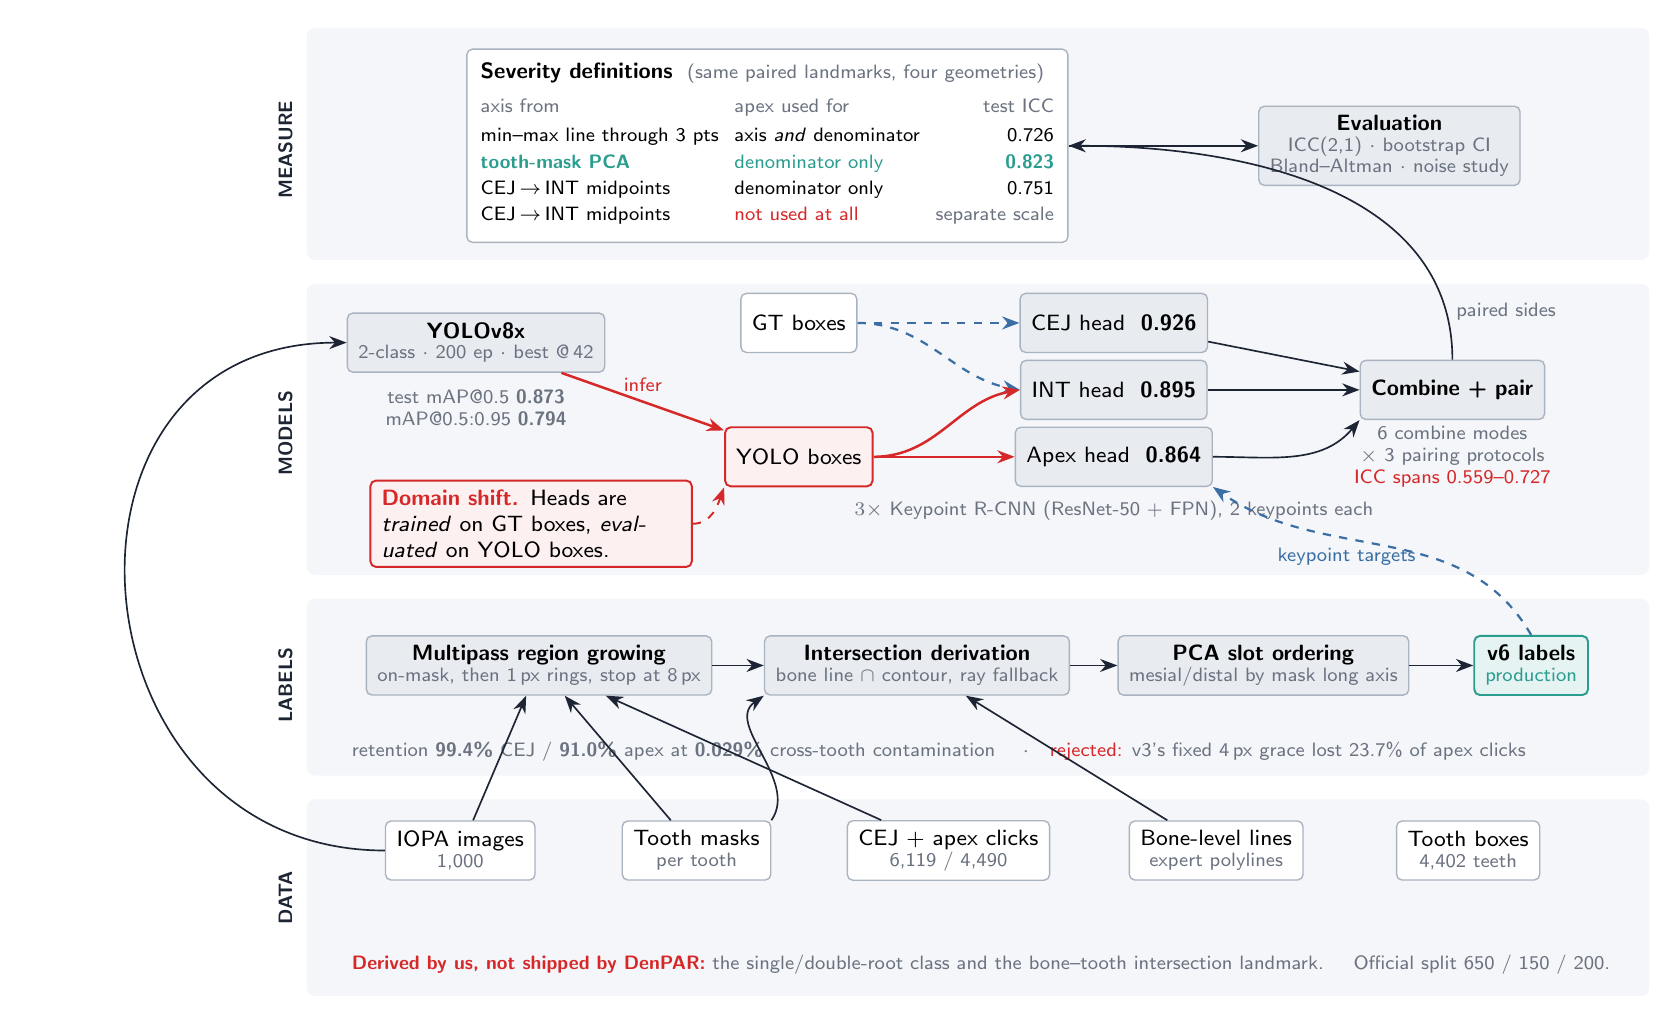
\begin{tikzpicture}[
  font=\sffamily\footnotesize,
  >={Stealth[length=2.2mm]},
  blk/.style={draw=edge,fill=white,rounded corners=2pt,minimum height=7.5mm,
              inner xsep=4pt,align=center,line width=0.5pt},
  proc/.style={blk,fill=soft},
  hl/.style={blk,fill=good!12,draw=good,line width=0.7pt},
  warn/.style={blk,fill=accent!7,draw=accent,line width=0.7pt},
  lbl/.style={font=\sffamily\scriptsize,text=muted,align=center},
  tag/.style={font=\sffamily\bfseries\scriptsize,text=ink},
  flow/.style={->,draw=ink,line width=0.6pt},
  trainflow/.style={->,draw=trainc,line width=0.8pt,dashed},
  infflow/.style={->,draw=accent,line width=0.9pt},
]

%========================= LANE BACKGROUNDS =========================
\begin{scope}[on background layer]
  \fill[lane,rounded corners=3pt] (0.15,-0.75) rectangle (17.2,1.75);
  \fill[lane,rounded corners=3pt] (0.15,2.05)  rectangle (17.2,4.30);
  \fill[lane,rounded corners=3pt] (0.15,4.60)  rectangle (17.2,8.30);
  \fill[lane,rounded corners=3pt] (0.15,8.60)  rectangle (17.2,11.55);
\end{scope}

\node[tag,rotate=90] at (-0.12,0.5)  {DATA};
\node[tag,rotate=90] at (-0.12,3.2)  {LABELS};
\node[tag,rotate=90] at (-0.12,6.4)  {MODELS};
\node[tag,rotate=90] at (-0.12,10.0) {MEASURE};

%========================= LANE 1 : DATA =========================
\node[blk] (img)    at (2.1,1.10)  {IOPA images\\[-2pt]\textcolor{muted}{\scriptsize 1{,}000}};
\node[blk] (masks)  at (5.1,1.10)  {Tooth masks\\[-2pt]\textcolor{muted}{\scriptsize per tooth}};
\node[blk] (clicks) at (8.3,1.10)  {CEJ + apex clicks\\[-2pt]\textcolor{muted}{\scriptsize 6{,}119 / 4{,}490}};
\node[blk] (bone)   at (11.7,1.10) {Bone-level lines\\[-2pt]\textcolor{muted}{\scriptsize expert polylines}};
\node[blk] (bbox)   at (14.9,1.10) {Tooth boxes\\[-2pt]\textcolor{muted}{\scriptsize 4{,}402 teeth}};

\node[lbl,anchor=west,align=left] at (0.6,-0.35)
  {\textcolor{accent}{\textbf{Derived by us, not shipped by DenPAR:}} the single/double-root class
   and the bone--tooth intersection landmark. \quad Official split 650 / 150 / 200.};

%========================= LANE 2 : LABEL CONSTRUCTION =========================
\node[proc] (rg)  at (3.1,3.45)  {\textbf{Multipass region growing}\\[-2pt]
      \textcolor{muted}{\scriptsize on-mask, then 1\,px rings, stop at 8\,px}};
\node[proc] (int) at (7.9,3.45)  {\textbf{Intersection derivation}\\[-2pt]
      \textcolor{muted}{\scriptsize bone line $\cap$ contour, ray fallback}};
\node[proc] (pca) at (12.3,3.45) {\textbf{PCA slot ordering}\\[-2pt]
      \textcolor{muted}{\scriptsize mesial/distal by mask long axis}};
\node[hl]   (v6)  at (15.7,3.45) {\textbf{v6 labels}\\[-2pt]\textcolor{good}{\scriptsize production}};

\node[lbl,anchor=west,align=left] at (0.6,2.35)
  {retention \textbf{99.4\%} CEJ / \textbf{91.0\%} apex at \textbf{0.029\%} cross-tooth contamination
   \quad$\cdot$\quad \textcolor{accent}{rejected:} v3's fixed 4\,px grace lost 23.7\% of apex clicks};

\draw[flow] (img)    -- (rg);
\draw[flow] (masks)  -- (rg);
\draw[flow] (clicks) -- (rg);
\draw[flow] (bone)   -- (int);
\draw[flow] (masks.north east) to[out=55,in=215] (int.south west);
\draw[flow] (rg) -- (int);
\draw[flow] (int) -- (pca);
\draw[flow] (pca) -- (v6);

%========================= LANE 3 : MODELS (the fork) =========================
\node[proc] (yolo)  at (2.3,7.55) {\textbf{YOLOv8x}\\[-2pt]
      \textcolor{muted}{\scriptsize 2-class $\cdot$ 200 ep $\cdot$ best @\,42}};
\node[lbl] at (2.3,6.72) {test mAP@0.5 \textbf{0.873}\\mAP@0.5:0.95 \textbf{0.794}};

\node[blk]  (gtbox) at (6.4,7.80) {GT boxes};
\node[warn] (yobox) at (6.4,6.10) {YOLO boxes};

\node[proc] (cej) at (10.4,7.80) {CEJ head\ \ \textbf{0.926}};
\node[proc] (ih)  at (10.4,6.95) {INT head\ \ \textbf{0.895}};
\node[proc] (ap)  at (10.4,6.10) {Apex head\ \ \textbf{0.864}};
\node[lbl]  at (10.4,5.42) {$3\times$ Keypoint R-CNN (ResNet-50 + FPN), 2 keypoints each};

\node[proc] (comb) at (14.7,6.95) {\textbf{Combine + pair}};
\node[lbl,align=center] at (14.7,6.10)
  {6 combine modes\\$\times$ 3 pairing protocols\\\textcolor{accent}{ICC spans 0.559--0.727}};

\draw[trainflow] (v6.north) to[out=120,in=-35] node[pos=0.62,below,lbl,text=trainc]{keypoint targets} (ap.south east);
\draw[trainflow] (gtbox) -- (cej);
\draw[trainflow] (gtbox.east) to[out=0,in=170] (ih.west);
\draw[infflow]   (yolo) -- node[pos=0.5,above,lbl,text=accent]{infer} (yobox);
\draw[infflow]   (yobox) -- (ap);
\draw[infflow]   (yobox.east) to[out=0,in=190] (ih.west);
\draw[flow] (cej) -- (comb);
\draw[flow] (ih)  -- (comb);
\draw[flow] (ap.east)  to[out=0,in=230] (comb.south west);
\draw[flow] (img.west) to[out=180,in=180,looseness=1.6] (yolo.west);

% The callout this figure exists for, placed in free space at lane left.
\node[warn,align=left,text width=38mm] (shift) at (3.0,5.25)
  {\textcolor{accent}{\textbf{Domain shift.}} Heads are \emph{trained} on GT boxes,
   \emph{evaluated} on YOLO boxes.};
\draw[->,draw=accent,dashed,line width=0.7pt] (shift.east) to[out=0,in=250] (yobox.south west);

%========================= LANE 4 : SEVERITY + EVALUATION =========================
% The four definitions are ALTERNATIVES over the same paired landmarks, so they are
% drawn as one comparison block rather than a chain.
\node[blk,align=left,inner sep=5pt] (sev) at (6.0,10.05) {%
  \textbf{Severity definitions} \;\textcolor{muted}{\scriptsize(same paired landmarks, four geometries)}\\[3pt]
  \begin{tabular}{@{}l@{\ \ }l@{\ \ }r@{}}
  \textcolor{muted}{\scriptsize axis from} & \textcolor{muted}{\scriptsize apex used for} & \textcolor{muted}{\scriptsize test ICC}\\[1pt]
  \scriptsize min--max line through 3 pts & \scriptsize axis \emph{and} denominator & \scriptsize 0.726\\
  \scriptsize\textcolor{good}{\textbf{tooth-mask PCA}} & \scriptsize\textcolor{good}{denominator only} & \scriptsize\textcolor{good}{\textbf{0.823}}\\
  \scriptsize CEJ\,$\to$\,INT midpoints & \scriptsize denominator only & \scriptsize 0.751\\
  \scriptsize CEJ\,$\to$\,INT midpoints & \scriptsize \textcolor{accent}{not used at all} & \scriptsize \textcolor{muted}{separate scale}\\
  \end{tabular}};

\node[proc] (ev) at (13.9,10.05) {\textbf{Evaluation}\\[-2pt]
      \textcolor{muted}{\scriptsize ICC(2,1) $\cdot$ bootstrap CI}\\[-2pt]
      \textcolor{muted}{\scriptsize Bland--Altman $\cdot$ noise study}};

\draw[flow] (comb.north) to[out=90,in=0] node[pos=0.10,right,lbl]{paired sides} (sev.east);
\draw[flow] (sev.east) -- (ev.west);

\end{tikzpicture}
\end{document}
